\begin{propertie}   Sean $U\subseteq \Rn{2}$ abierto  y   $D \subsetneq  U$ un conjunto  simplemente conexo  cuyo borde, $\partial D$, es una curva simple, cerrada y suave a trozos.  Si  $\mathbf{F}:U\to\Rn{2}$ tal que $ \grad\times\mathbf{F} =1 $ entonces
    \[
        \oint_{\partial D^{+}} \mathbf{F}\cdot d\mathbf{s} =  \text{Área}(D).
    \]
\end{propertie}

\begin{tarea}
Hallar el \'area de la regi\'on encerrada por la curva cerrada con parametrizaci\'on   $\sigma(t) = (\sin t \cos t, \sin t)$ con $0\leq t \leq \pi$.     

\begin{figure}[H]
\begin{center}
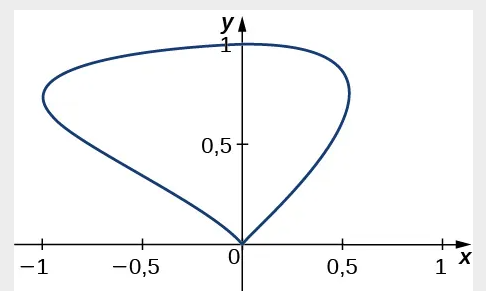
\includegraphics[scale=0.6]{figs/green.png}
\end{center}
\end{figure}
\end{tarea}